\documentclass{beamer}
\mode<presentation>

\setbeamertemplate{navigation symbols}{}

\usetheme{Madrid}
\usecolortheme{dove}

\usepackage[italian]{babel}
\usepackage{graphicx}
\usepackage{import}
\usepackage{color}
\usepackage{framed}
\usepackage[utf8]{inputenc}
\usepackage{hyperref}

\author{Marco Melletti}
\title{uARM: a simple ARM virtual machine}

\begin{document}

\begin{frame}
        \titlepage
\end{frame}

\begin{frame}{Genealogia delle VM}
\begin{itemize}\itemsep20pt
\item Chip: PDP-11, device ancora utilizzati (1983)
\item MPS: MIPS, memoria virtuale sempre attiva (2004)
\item uMPS: MIPS, memoria virtuale opzionale (2007)
\item uMPS2: MIPS, supp orto multicore, interfaccia grafica ristrutturata (2011)
\item uARM
\end{itemize}
\end{frame}

\begin{frame}{ARM: Advanced RISC Machine}
\begin{itemize}\itemsep20pt
\item Architettura RISC: Reduced Instruction Set Computer
\item Attuale e largamente utilizzata:

	\begin{itemize}\itemsep4pt
	\item Embedded Systems
	\item Smartphones
	\item Nintendo DS
	\item Raspb erry Pi
	\item Game Boy Advance
	\item iPod
	\item ...
	\end{itemize}
\end{itemize}
\end{frame}

\begin{frame}{uARM}
\begin{itemize}\itemsep10pt
\item Processore ARM7TDMI
\item Memoria Little-Endian a dimensione variabile
\item MMU con TLB a dimensione variabile
\item 8 Device per tipo:

	\begin{itemize}\itemsep4pt
	\item terminali
	\item stampanti
	\item schede di rete (VDE)
	\item dischi fissi
	\item nastri (dischi ottici)
	\end{itemize}
\end{itemize}
\end{frame}

\begin{frame}{uARM: GUI}
\centering
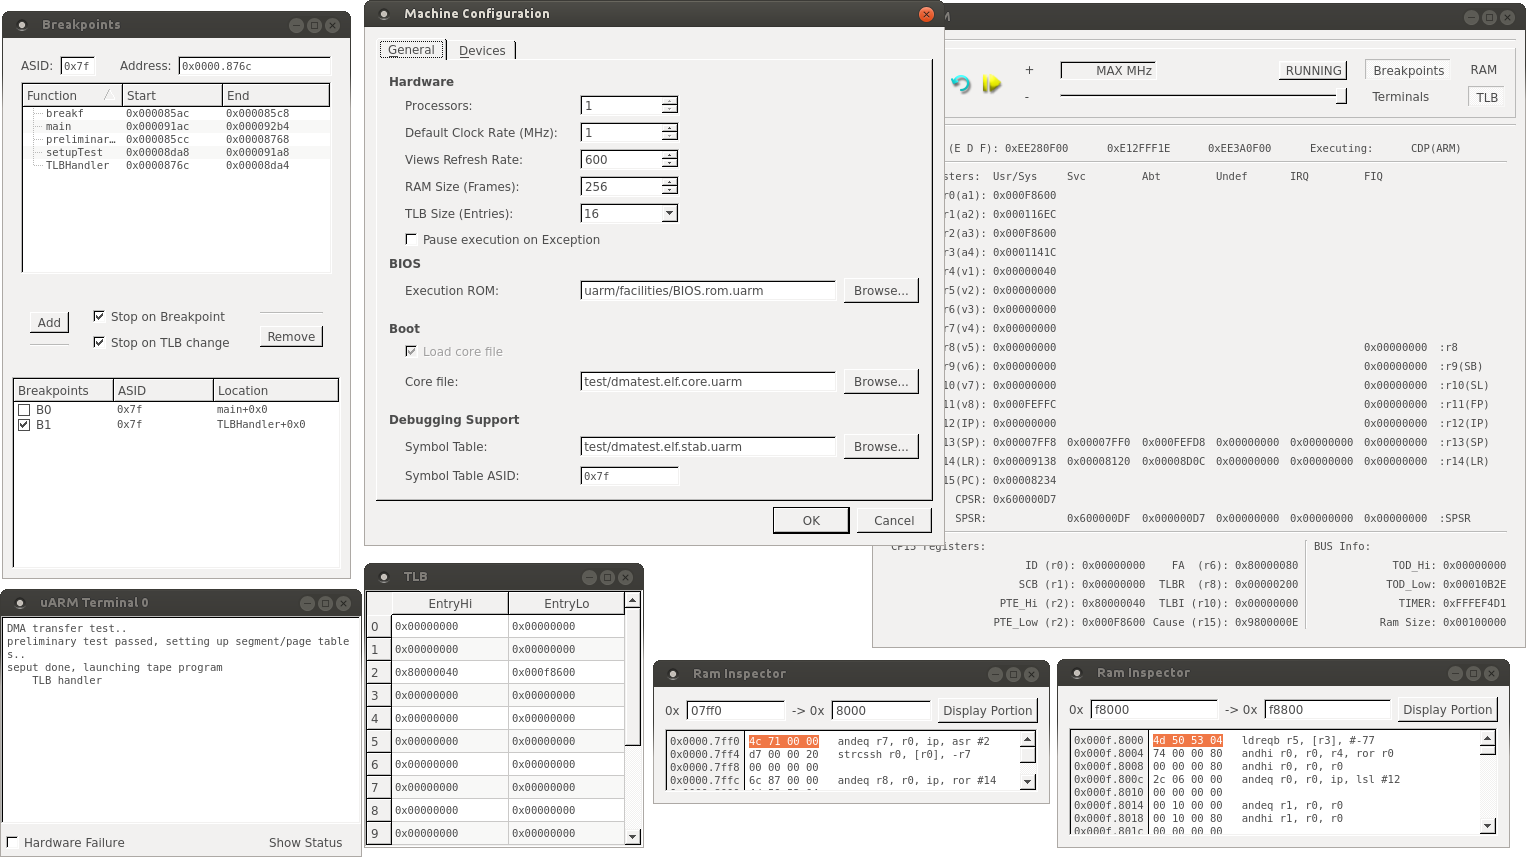
\includegraphics[width=\textwidth]{img/gui_completa.png}
\end{frame}

\begin{frame}{uARM: GUI}
\begin{center}
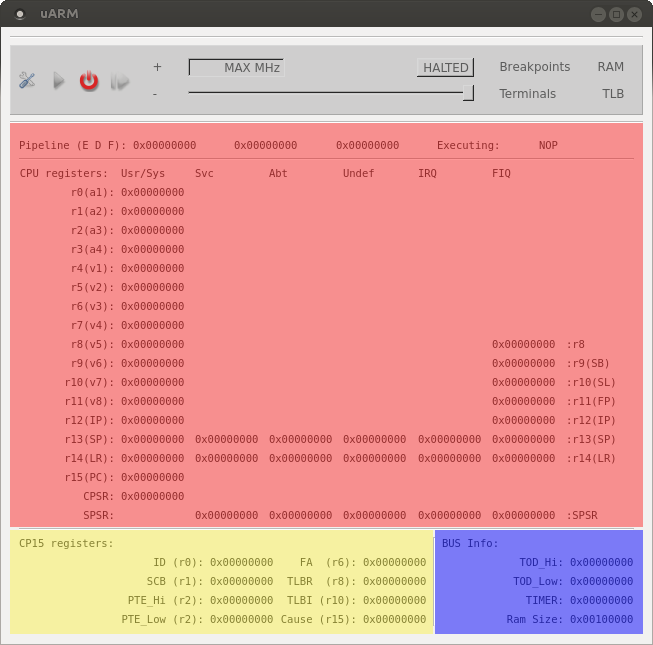
\includegraphics[height=0.6\textheight]{img/gui_colori.png}
\end{center}

{\footnotesize
\begin{itemize}\itemsep1pt
\item \textcolor{gray}{Barra di controllo}
\item \textcolor{red}{Stato Processore}
\item \textcolor{yellow}{Stato Coprocessore}
\item \textcolor{blue}{Informazioni di sistema}
\end{itemize}}
\end{frame}

\begin{frame}{uARM: Barra di controllo}

\begin{center}
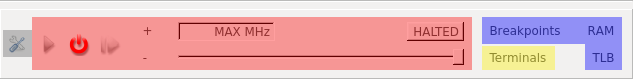
\includegraphics[width=0.85\textwidth]{img/controllo_colori.png}
\end{center}

\vfill

{\footnotesize
\begin{itemize}\itemsep1pt
\item \textcolor{gray}{Configurazioni}
\item \textcolor{red}{Controllo esecuzione}
\item \textcolor{yellow}{Terminali}
\item \textcolor{blue}{Funzioni di debug}
\end{itemize}}
\end{frame}

\begin{frame}{uARM: un esempio}
Sorgente: \texttt{foo/esempio.c}

\vspace{20px}
\begin{framed}
\small\texttt{\#include /usr/include/uarm/libuarm.h\newline
\newline
int main()\{\\
~~~~tprint("Hellp World$\backslash$n$\backslash$0");\\
~~~~HALT();\\
~~~~tprint("");\\
~~~~return 0;\\
\} }
\end{framed}
\end{frame}

\begin{frame}{Compilazione: un esempio}
Sorgente: \texttt{foo/esempio.c}

\vspace{15px}
Compiliamo il file:\\
{\small\texttt{\$> arm-none-eabi-gcc -mcpu=arm7tdmi -c -o foo/esempio.o $\backslash$
\\foo/esempio.c}}

\vspace{15px}
Linkiamo il file oggetto con la libreria di uARM e il file di inzializzazione:\\
{\small\texttt{\$> arm-none-eabi-ld -T $\backslash$\\
/usr/include/uarm/ldscripts/elf32ltsarm.h.uarmcore.x $\backslash$\\
-o esempio.elf /usr/include/uarm/crtso.o $\backslash$\\
/usr/include/uarm/libuarm.o esempio.o}}

\vspace{15px}
Convertiamo l'eseguibile nel formato di uARM:\\
{\small\texttt{\$> elf2uarm -k foo/esempio.elf}}

\end{frame}

\begin{frame}{Esecuzione: un esempio}
Impostiamo il core file generato per l'esecuzione:
\newline

\centering
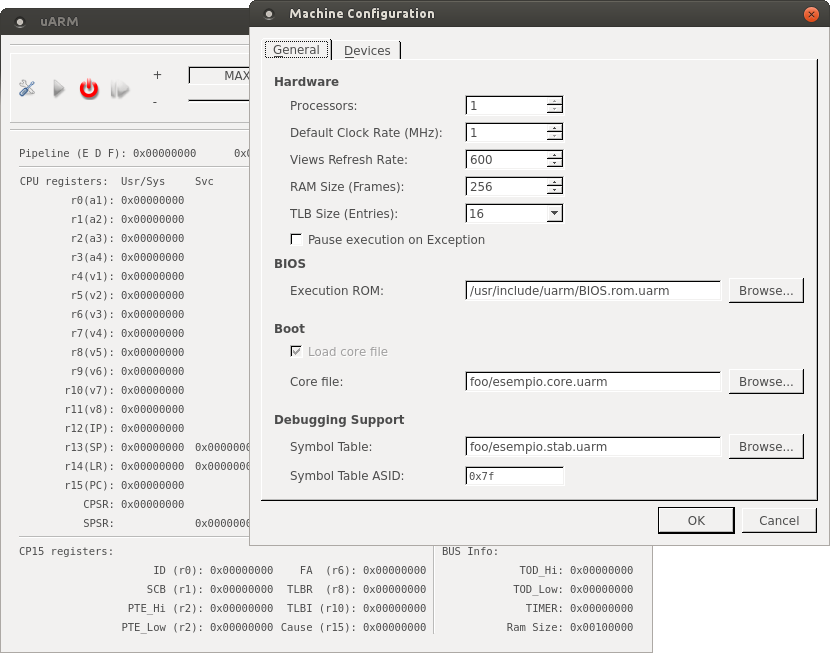
\includegraphics[height=0.75\textheight]{img/esempio_config.png}
\end{frame}

\begin{frame}{Esecuzione: un esempio}
Avviamo la macchina e lanciamo l'esecuzione, il terminale 0 mostrerà l'output:

\centering
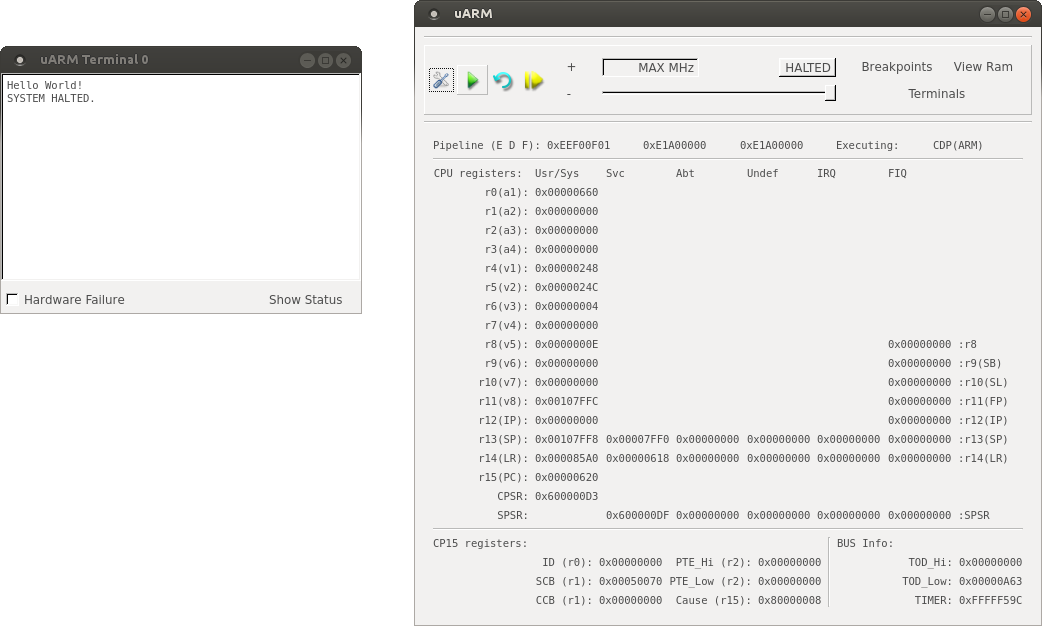
\includegraphics[height=0.75\textheight]{img/esempio_exec.png}
\end{frame}

\begin{frame}{uARM: un altro esempio}
\Large Proviamo davvero la maccina...
\end{frame}

\begin{frame}{uARM}
\begin{itemize}\itemsep25pt
\item Home page: \url{http://mellotanica.github.io/uARM/}

	\begin{itemize}\itemsep5pt
	\item Repository ufficiale
	\item Pacchetti per VirtLab
	\item Questa introduzione
	\item Specifiche della macchina
	\end{itemize}
	
\item Contattatemi per domande/problemi/richieste

	\begin{itemize}\itemsep4pt
	\item marco.melletti@studio.unibo.it
	\item mellotanica@hotmail.it
	\end{itemize}
\end{itemize}
\end{frame}

\begin{frame}{Grazie dell'attenzione}
\begin{center}\huge 
Domande?
\end{center}
\end{frame}

\end{document}